
        \documentclass[12p]{article}
        \usepackage[margin=1in, left=1.5in, includefoot]{geometry}
        \usepackage{longtable, tabu}
        \usepackage[table, dvipsnames]{xcolor}
        \usepackage{array,booktabs}
        \usepackage{color}
        \usepackage{indentfirst}
        \usepackage{graphicx}
        \usepackage{float}
        \usepackage[utf8]{inputenc}
        \usepackage{listings}
        \usepackage{url}
        \usepackage{multirow}
        \usepackage{seqsplit}
        
        \definecolor{ferrarired}{rgb}{1.0, 0.11, 0.0}
        \definecolor{orange(colorwheel)}{rgb}{1.0, 0.5, 0.0}
        \definecolor{deepskyblue}{rgb}{0.0, 0.75, 1.0}
        \definecolor{grannysmithapple}{rgb}{0.66, 0.89, 0.63}
        \definecolor{gray(x11gray)}{rgb}{0.75, 0.75, 0.75}
        \definecolor{amber}{rgb}{1.0, 0.75, 0.0}
        
        \newcommand{\icon}[1]{\includegraphics[height=12pt]{#1}}
        \newcommand{\hash}[1]{{\ttfamily\seqsplit{#1}}}

        \setlength{\arrayrulewidth}{0.3mm}
\setlength{\tabcolsep}{18pt}
\renewcommand{\arraystretch}{1.5}
\setlength{\parindent}{1em}
\begin{document}
\begin{titlepage}
\begin{center}
\line(1,0){320}\\
[0.25in]
\huge{\bfseries Android Analysis Report}
\line(1,0){320}\\
[0.5in]
\begin{figure}[H]
	\centering
	
\includegraphics[scale=0.5]{/home/miki/Documents/GITHUB/AndroidPermissions/python/vulns/report_icons/logo.png}
\end{figure}
\textsl{\LARGE Demo app}\\
\textsf{\LARGE com.kbank.otp}\\
[2.5in]
\end{center}
\begin{flushright}
\textbf{\large Date 2018-06-14}
\end{flushright}
\end{titlepage}
\tableofcontents
\thispagestyle{empty}
\cleardoublepage
\setcounter{page}{1}
\section{PERMISSIONS}
	\begin{longtable}{p{3cm} p{10cm} }
	\rowcolor{grannysmithapple!70} Type & List \\
Normal &  ACCESS\_NETWORK\_STATE \\ 
 &  INTERNET \\ 
 &  WAKE\_LOCK \\ 
\hline
Dangerous &  ACCESS\_COARSE\_LOCATION \\ 
 &  ACCESS\_FINE\_LOCATION \\ 
 &  WRITE\_EXTERNAL\_STORAGE \\ 
\hline
Overprivileged &  READ\_EXTERNAL\_STORAGE \\ 
 &  C \\ 
 &  MAPS\_RECEIVE \\ 
 &  ACCESS\_WIFI\_STATE \\ 
 &  RECEIVE \\ 
 &  READ\_GSERVICES \\ 
 &  ACCESS\_DOWNLOAD\_MANAGER \\ 
 &  READ\_PHONE\_STATE \\ 
\hline
Underprivileged &  "android.permission.INTERNET" \\ 
 &  "android.permission.ACCESS\_COARSE\_LOCATION" \\ 
 &  UPDATE\_DEVICE\_STATS \\ 
 &  "android.permission.WAKE\_LOCK" \\ 
 &  "android.permission.ACCESS\_NETWORK\_STATE" \\ 
 &  "android.permission.ACCESS\_FINE\_LOCATION" \\ 
\hline
Automatically granted dangerous permissions &  ANSWER\_PHONE\_CALLSREAD\_PHONE\_NUMBERS \\ 
 &  CALL\_PHONE \\ 
 &  READ\_CALL\_LOG \\ 
 &  WRITE\_CALL\_LOG \\ 
 &  ADD\_VOICEMAIL \\ 
 &  USE\_SIP \\ 
 &  PROCESS\_OUTGOING\_CALLS \\ 
\hline
	\end{longtable}
\section{FINDINGS SUMMARY}\label{sec:summary}
\begin{figure}[H]
\centering
	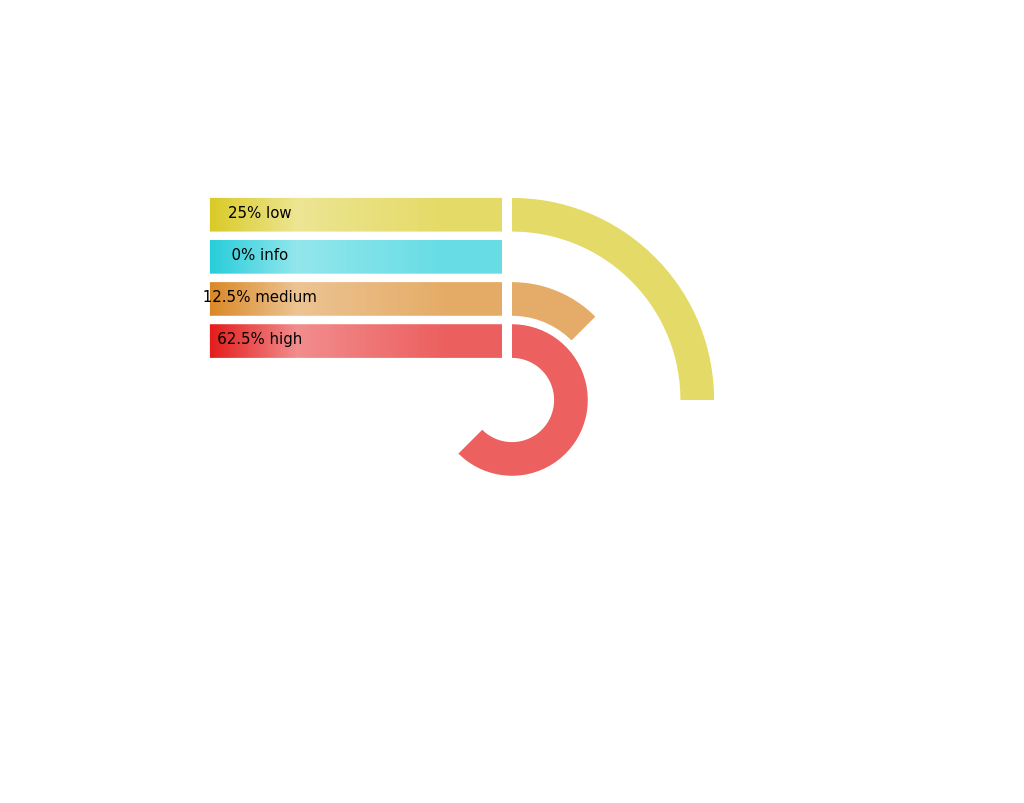
\includegraphics[scale=0.5]{/home/miki/Documents/GITHUB/AndroidPermissions/apks/playstore_apps/com_kbank_otp/report/pie_chart.png}
\end{figure}
	\begin{longtable}{p{0.5cm} p{10cm} p{1.5cm}}
	\rowcolor{grannysmithapple!70} Index & Title & Impact \\
	A1&& \color{amber}\textbf{Low} \\
\hline\\	A2&Application Data can be Backed up& \color{orange(colorwheel)}\textbf{Medium} \\
\hline\\	A3&Launch Mode of Activity \newline (com. kbank. otp. MainActivity) is not standard.& \color{ferrarired}\textbf{High} \\
\hline\\	A4&Activity \newline (com. kbank. otp. MainActivity) is not Protected. An intent-filter exists.& \color{ferrarired}\textbf{High} \\
\hline\\	A5&Service \newline (com. kbank. otp. services. FirebaseMessagingService) is not Protected. An intent-filter exists.& \color{ferrarired}\textbf{High} \\
\hline\\	A6&Service \newline (com. kbank. otp. services. FirebaseInstanceIDService) is not Protected. An intent-filter exists.& \color{ferrarired}\textbf{High} \\
\hline\\	A7&Service \newline (com. google. firebase. messaging. FirebaseMessagingService) is not Protected. [android:exported=true]& \color{ferrarired}\textbf{High} \\
\hline\\	A8&Service \newline (com. google. firebase. iid. FirebaseInstanceIdService) is not Protected. [android:exported=true]& \color{ferrarired}\textbf{High} \\
\hline\\	A9&& \color{amber}\textbf{Low} \\
\hline\\	\end{longtable}
\cleardoublepage
\newpage
\section{DETAILED FINDINGS}
\subsection{A1: }
\subsubsection*{\protect\icon{/home/miki/Documents/GITHUB/AndroidPermissions/python/vulns/report_icons/basic_sheet.png} Description}

\subsubsection*{\protect\icon{/home/miki/Documents/GITHUB/AndroidPermissions/python/vulns/report_icons/basic_magnifier.png} Evidence}
\path{/home/miki/Documents/GITHUB/AndroidPermissions/apks/playstore_apps/com_kbank_otp/app/smali/android/support/v4/text/ICUCompatIcs.smali
Landroid/util/Log -> w(Ljava/lang/String;Ljava/lang/Throwable;)}

\path{/home/miki/Documents/GITHUB/AndroidPermissions/apks/playstore_apps/com_kbank_otp/app/smali/android/support/v4/text/ICUCompatIcs.smali
Landroid/util/Log -> w(Ljava/lang/String;Ljava/lang/Throwable;)}

\path{/home/miki/Documents/GITHUB/AndroidPermissions/apks/playstore_apps/com_kbank_otp/app/smali/android/support/v4/text/ICUCompatIcs.smali
Landroid/util/Log -> w(Ljava/lang/String;Ljava/lang/Throwable;)}

\path{/home/miki/Documents/GITHUB/AndroidPermissions/apks/playstore_apps/com_kbank_otp/app/smali/android/support/v4/text/ICUCompatIcs.smali
Landroid/util/Log -> w(Ljava/lang/String;Ljava/lang/Throwable;)}

\path{/home/miki/Documents/GITHUB/AndroidPermissions/apks/playstore_apps/com_kbank_otp/app/smali/android/support/v4/text/ICUCompatIcs.smali
Landroid/util/Log -> w(Ljava/lang/String;Ljava/lang/Throwable;)}

\path{/home/miki/Documents/GITHUB/AndroidPermissions/apks/playstore_apps/com_kbank_otp/app/smali/android/support/v4/text/ICUCompatApi23.smali
Landroid/util/Log -> w(Ljava/lang/String;Ljava/lang/Throwable;)}

\path{/home/miki/Documents/GITHUB/AndroidPermissions/apks/playstore_apps/com_kbank_otp/app/smali/android/support/v4/text/ICUCompatApi23.smali
Landroid/util/Log -> w(Ljava/lang/String;Ljava/lang/Throwable;)}

\path{/home/miki/Documents/GITHUB/AndroidPermissions/apks/playstore_apps/com_kbank_otp/app/smali/android/support/v4/print/PrintHelperKitkat.smali
Landroid/util/Log -> w(Ljava/lang/String;Ljava/lang/String;Ljava/lang/Throwable;)}

\path{/home/miki/Documents/GITHUB/AndroidPermissions/apks/playstore_apps/com_kbank_otp/app/smali/android/support/v4/print/PrintHelperKitkat.smali
Landroid/util/Log -> w(Ljava/lang/String;Ljava/lang/String;Ljava/lang/Throwable;)}

\path{/home/miki/Documents/GITHUB/AndroidPermissions/apks/playstore_apps/com_kbank_otp/app/smali/android/support/v4/print/PrintHelperKitkat.smali
Landroid/util/Log -> e(Ljava/lang/String;Ljava/lang/String;Ljava/lang/Throwable;)}


\textit{snip}
\newline \textsl{For the full list view \path{/home/miki/Documents/GITHUB/AndroidPermissions/apks/playstore_apps/com_kbank_otp/report}}
\subsubsection*{\protect\icon{/home/miki/Documents/GITHUB/AndroidPermissions/python/vulns/report_icons/basic_todo.png} Recommendation}

\subsection{A2: Application Data can be Backed up}
\subsubsection*{\protect\icon{/home/miki/Documents/GITHUB/AndroidPermissions/python/vulns/report_icons/basic_sheet.png} Description}
This flag allows anyone to backup your application data via adb. It allows users who have enabled USB debugging to copy application data off of the device.
\subsubsection*{\protect\icon{/home/miki/Documents/GITHUB/AndroidPermissions/python/vulns/report_icons/basic_todo.png} Recommendation}
android:allowBackup = False
\subsection{A3: Launch Mode of Activity (com. kbank. otp. MainActivity) is not standard.}
\subsubsection*{\protect\icon{/home/miki/Documents/GITHUB/AndroidPermissions/python/vulns/report_icons/basic_sheet.png} Description}
An Activity should not be having the launch mode attribute set to "singleTask/singleInstance" as it becomes root Activity and it is possible for other applications to read the contents of the calling Intent.
\subsubsection*{\protect\icon{/home/miki/Documents/GITHUB/AndroidPermissions/python/vulns/report_icons/basic_todo.png} Recommendation}
It is required to use the "standard" launch mode attribute when sensitive information is included in an Intent.
\subsection{A4: Activity (com. kbank. otp. MainActivity) is not Protected. An intent-filter exists.}
\subsubsection*{\protect\icon{/home/miki/Documents/GITHUB/AndroidPermissions/python/vulns/report_icons/basic_sheet.png} Description}
A  Activity is found to be shared with other apps on the device therefore leaving it accessible to any other application on the device. The presence of intent-filter indicates that the Activity is explicitly exported.
\subsubsection*{\protect\icon{/home/miki/Documents/GITHUB/AndroidPermissions/python/vulns/report_icons/basic_todo.png} Recommendation}
It is recommended to set the protection level to signature, so only applications signed with the same certificate can obtain the permission.
\subsection{A5: Service (com. kbank. otp. services. FirebaseMessagingService) is not Protected. An intent-filter exists.}
\subsubsection*{\protect\icon{/home/miki/Documents/GITHUB/AndroidPermissions/python/vulns/report_icons/basic_sheet.png} Description}
A  Service is found to be shared with other apps on the device therefore leaving it accessible to any other application on the device. The presence of intent-filter indicates that the Service is explicitly exported.
\subsubsection*{\protect\icon{/home/miki/Documents/GITHUB/AndroidPermissions/python/vulns/report_icons/basic_todo.png} Recommendation}
It is recommended to set the protection level to signature, so only applications signed with the same certificate can obtain the permission.
\subsection{A6: Service (com. kbank. otp. services. FirebaseInstanceIDService) is not Protected. An intent-filter exists.}
\subsubsection*{\protect\icon{/home/miki/Documents/GITHUB/AndroidPermissions/python/vulns/report_icons/basic_sheet.png} Description}
A  Service is found to be shared with other apps on the device therefore leaving it accessible to any other application on the device. The presence of intent-filter indicates that the Service is explicitly exported.
\subsubsection*{\protect\icon{/home/miki/Documents/GITHUB/AndroidPermissions/python/vulns/report_icons/basic_todo.png} Recommendation}
It is recommended to set the protection level to signature, so only applications signed with the same certificate can obtain the permission.
\subsection{A7: Service (com. google. firebase. messaging. FirebaseMessagingService) is not Protected. [android:exported=true]}
\subsubsection*{\protect\icon{/home/miki/Documents/GITHUB/AndroidPermissions/python/vulns/report_icons/basic_sheet.png} Description}
A Service is found to be shared with other apps on the device therefore leaving it accessible to any other application on the device.
\subsubsection*{\protect\icon{/home/miki/Documents/GITHUB/AndroidPermissions/python/vulns/report_icons/basic_todo.png} Recommendation}
It is recommended to set the protection level to signature, so only applications signed with the same certificate can obtain the permission.
\subsection{A8: Service (com. google. firebase. iid. FirebaseInstanceIdService) is not Protected. [android:exported=true]}
\subsubsection*{\protect\icon{/home/miki/Documents/GITHUB/AndroidPermissions/python/vulns/report_icons/basic_sheet.png} Description}
A Service is found to be shared with other apps on the device therefore leaving it accessible to any other application on the device.
\subsubsection*{\protect\icon{/home/miki/Documents/GITHUB/AndroidPermissions/python/vulns/report_icons/basic_todo.png} Recommendation}
It is recommended to set the protection level to signature, so only applications signed with the same certificate can obtain the permission.
\subsection{A9: }
\subsubsection*{\protect\icon{/home/miki/Documents/GITHUB/AndroidPermissions/python/vulns/report_icons/basic_sheet.png} Description}

\subsubsection*{\protect\icon{/home/miki/Documents/GITHUB/AndroidPermissions/python/vulns/report_icons/basic_magnifier.png} Evidence}
\path{/home/miki/Documents/GITHUB/AndroidPermissions/apks/playstore_apps/com_kbank_otp/app/smali/android/support/v4/text/ICUCompatIcs.smali forName}

\path{/home/miki/Documents/GITHUB/AndroidPermissions/apks/playstore_apps/com_kbank_otp/app/smali/android/support/v4/text/ICUCompatIcs.smali invoke}

\path{/home/miki/Documents/GITHUB/AndroidPermissions/apks/playstore_apps/com_kbank_otp/app/smali/android/support/v4/text/ICUCompatIcs.smali invoke}

\path{/home/miki/Documents/GITHUB/AndroidPermissions/apks/playstore_apps/com_kbank_otp/app/smali/android/support/v4/text/ICUCompatApi23.smali forName}

\path{/home/miki/Documents/GITHUB/AndroidPermissions/apks/playstore_apps/com_kbank_otp/app/smali/android/support/v4/text/ICUCompatApi23.smali invoke}

\path{/home/miki/Documents/GITHUB/AndroidPermissions/apks/playstore_apps/com_kbank_otp/app/smali/android/support/v4/util/MapCollections.smali getComponentType}

\path{/home/miki/Documents/GITHUB/AndroidPermissions/apks/playstore_apps/com_kbank_otp/app/smali/android/support/v4/graphics/drawable/DrawableCompatJellybeanMr1.smali invoke}

\path{/home/miki/Documents/GITHUB/AndroidPermissions/apks/playstore_apps/com_kbank_otp/app/smali/android/support/v4/graphics/drawable/DrawableCompatJellybeanMr1.smali invoke}

\path{/home/miki/Documents/GITHUB/AndroidPermissions/apks/playstore_apps/com_kbank_otp/app/smali/android/support/v4/app/BundleCompatDonut.smali invoke}

\path{/home/miki/Documents/GITHUB/AndroidPermissions/apks/playstore_apps/com_kbank_otp/app/smali/android/support/v4/app/BundleCompatDonut.smali invoke}


\textit{snip}
\newline \textsl{For the full list view \path{/home/miki/Documents/GITHUB/AndroidPermissions/apks/playstore_apps/com_kbank_otp/report}}
\subsubsection*{\protect\icon{/home/miki/Documents/GITHUB/AndroidPermissions/python/vulns/report_icons/basic_todo.png} Recommendation}

\cleardoublepage
\newpage
\section{VISUALIZATIONS}
\subsection{Chord Diagram - Class Relations}
\begin{figure}[H]
	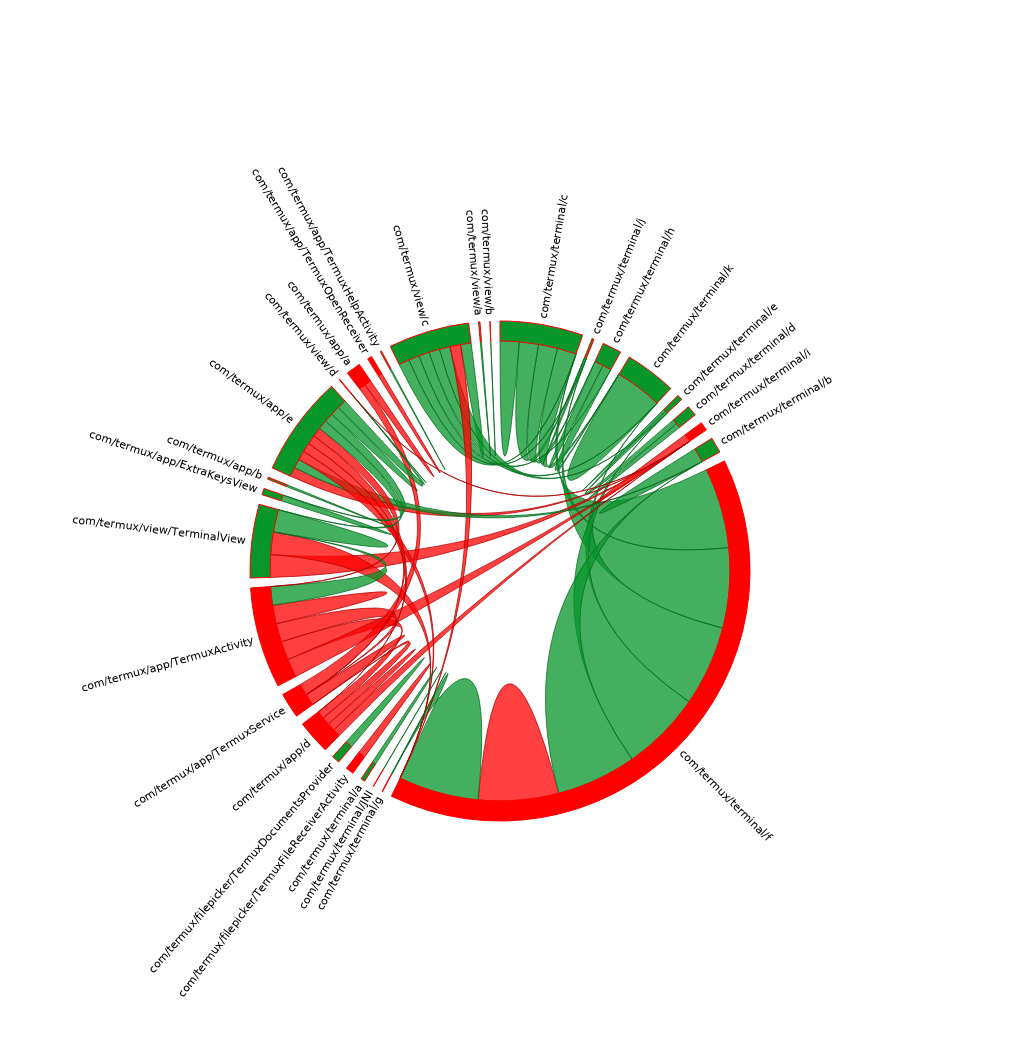
\includegraphics[scale=0.45]{/home/miki/Documents/GITHUB/AndroidPermissions/apks/playstore_apps/com_kbank_otp/report/chord_diagram.png}\end{figure}\subsection{Hot Spot - System Overview}
\begin{figure}[H]
\centering
	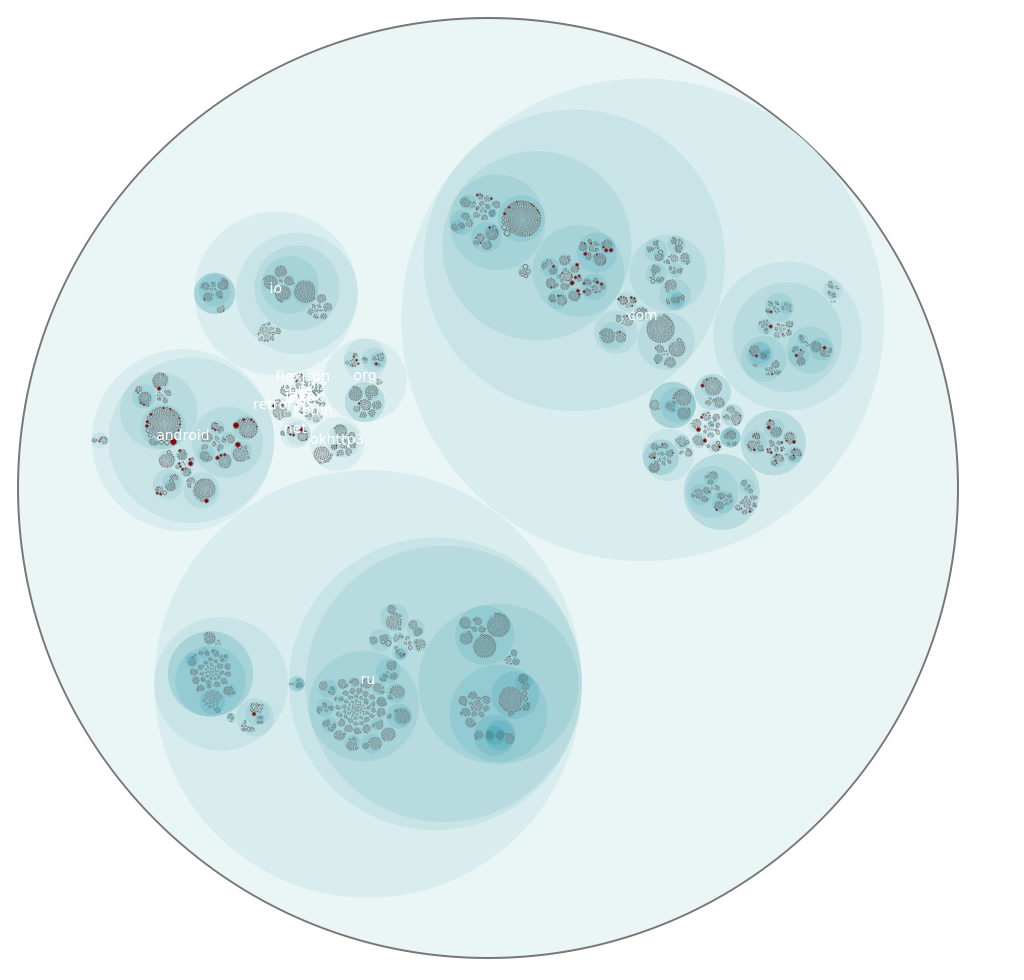
\includegraphics[scale=0.5]{/home/miki/Documents/GITHUB/AndroidPermissions/apks/playstore_apps/com_kbank_otp/report/hotspot.png}\end{figure}\begin{longtable}{p{0.3cm} p{12cm}}
\rowcolor{orange} Index & Class \\
1 & \path{/home/miki/Documents/GITHUB/AndroidPermissions/apks/playstore_apps/com_kbank_otp/app/smali/android/support/v4/media/MediaBrowserCompat$MediaBrowserImplBase.smali} \\
2 & \path{/home/miki/Documents/GITHUB/AndroidPermissions/apks/playstore_apps/com_kbank_otp/app/smali/com/google/firebase/iid/zzf.smali} \\
3 & \path{/home/miki/Documents/GITHUB/AndroidPermissions/apks/playstore_apps/com_kbank_otp/app/smali/android/support/v4/media/session/MediaControllerCompat$TransportControlsBase.smali} \\
4 & \path{/home/miki/Documents/GITHUB/AndroidPermissions/apks/playstore_apps/com_kbank_otp/app/smali/android/support/v4/media/session/MediaControllerCompat$MediaControllerImplBase.smali} \\
5 & \path{/home/miki/Documents/GITHUB/AndroidPermissions/apks/playstore_apps/com_kbank_otp/app/smali/com/google/android/gms/internal/zztl.smali} \\
6 & \path{/home/miki/Documents/GITHUB/AndroidPermissions/apks/playstore_apps/com_kbank_otp/app/smali/android/support/v4/app/NotificationManagerCompat$SideChannelManager.smali} \\
7 & \path{/home/miki/Documents/GITHUB/AndroidPermissions/apks/playstore_apps/com_kbank_otp/app/smali/com/google/android/gms/common/internal/zzg.smali} \\
8 & \path{/home/miki/Documents/GITHUB/AndroidPermissions/apks/playstore_apps/com_kbank_otp/app/smali/android/support/v7/widget/SuggestionsAdapter.smali} \\
9 & \path{/home/miki/Documents/GITHUB/AndroidPermissions/apks/playstore_apps/com_kbank_otp/app/smali/com/google/android/gms/common/zze.smali} \\
10 & \path{/home/miki/Documents/GITHUB/AndroidPermissions/apks/playstore_apps/com_kbank_otp/app/smali/com/google/firebase/iid/FirebaseInstanceIdService.smali} \\
	\end{longtable}
\end{document}
